\documentclass[a5paper,11pt]{memoir}
% TODO try this booklet feature
% https://tex.stackexchange.com/a/17008/133684
% \usepackage{pdfpages}
% \documentclass[17pt]{memoir}
\usepackage[T2A,T1]{fontenc}
\usepackage[utf8]{inputenc}
\usepackage[russian]{babel}
\usepackage{multicol}
\usepackage{hyperref}
\usepackage[math]{anttor}  % set font to Antykwa Torunska
\usepackage[pages=some]{background}
\usepackage{fancyhdr}  % needed to omit chapter name on every page
\usepackage{menukeys}  % for keyboard shortcuts rendered in a special style
\usepackage[symbol]{footmisc} % for dagger footnote
\usepackage{wrapfig}
\usepackage{subcaption} % for displaying figures side by side
\usepackage{geometry}
\usepackage{fontawesome5}

\usepackage{yfonts,color}

\usepackage{iftex} % for identifying luatex and pdftex

\ifluatex
	% we're building the special version for dyslexics, it uses a different
	% font; this can only be done with LuaLaTeX, so we wrap with an #ifdef-like
	% structure; this logic only applies when compiling with lualatex, otherwise
	% the typical pdflatex approach is taken
	
	% the font has to be copied to /usr/share/fonts/opentype/adys
	\usepackage{fontspec}
	\setmainfont{Adys}
\fi


% \usepackage{nextpage} % needed for \cleartoevenpage, to ensure the last page/cover will fold as we need

% this is to have proper quotes for Russian text <<  >> (not " ")
\usepackage{csquotes}


\newif\ifincludetranslations
\includetranslationstrue % Uncomment this line to include translations.tex




% Syntactic sugar: a command for direct speech of various characters - it will be rendered as
% a quote with an emphasis. For quoting non-speech, use \textquote
\newcommand{\say}[1]{\emph{\textquote{#1}}}


% this is used to set the metadata of the PDF itself
% see https://en.wikibooks.org/wiki/LaTeX/Hyperlinks#Customization
\hypersetup{
    pdftitle={0! Рассказы о тех, кто не заблудился},
    pdfauthor={Alex Railean},
    pdfsubject={Рассказы для детей},
    % pdfcreator={Creator},   % creator of the document
    % pdfproducer={Producer}, % producer of the document
    pdfkeywords={рассказы, образование}, % list of keywords
    pdfpagelayout=TwoPageRight, % display as 2 columns by default, useful during development and testing
}



% EXPERIMENT with this to manipulate margin size
% https://tex.stackexchange.com/a/378157/133684
% \setlrmarginsandblock{3.5cm}{2.5cm}{*}
% \setulmarginsandblock{2.5cm}{*}{1}
% \checkandfixthelayout 


\title{\begin{otherlanguage*}{russian}
0! Рассказы о тех, кто не заблудился
\end{otherlanguage*}}  
% \author{Alex Railean}
\author{}
% \date{November 2022}


% This is necessary to remove chapter titles from every page, which would be shown otherwise
% https://stackoverflow.com/a/62250429/27342
\pagestyle{fancy}
\fancyhead[R]{\thepage}
\fancyhead[L]{}
\renewcommand{\headrulewidth}{0pt}
\fancyfoot{}
%%%%%%%%%%%%%%%%%%%%%%%%%%%%%%%%%%%%%%%%%%%%



% Adjust poem titles, so they are bigger and thicker
\renewcommand{\PoemTitlefont}{%
\normalfont\huge\bfseries\centering}


% Set the right margin to 1cm and the top margin to 1.5cm.
% https://tex.stackexchange.com/a/378157/133684
\setlrmarginsandblock{*}{1cm}{1}
\setulmarginsandblock{1.5cm}{*}{1}
\checkandfixthelayout
\begin{document}
% redefine font size 14 as 14.5 using this method, because doing it at the very top of the file only lets us choose between 12 14 17...
% https://tex.stackexchange.com/questions/323443/how-to-specify-intermediate-font-sizes-in-memoir-class
% \fontsize{15pt}{14pt}\selectfont

\date{} % so no date is shown under the title
\maketitle
\begin{center}
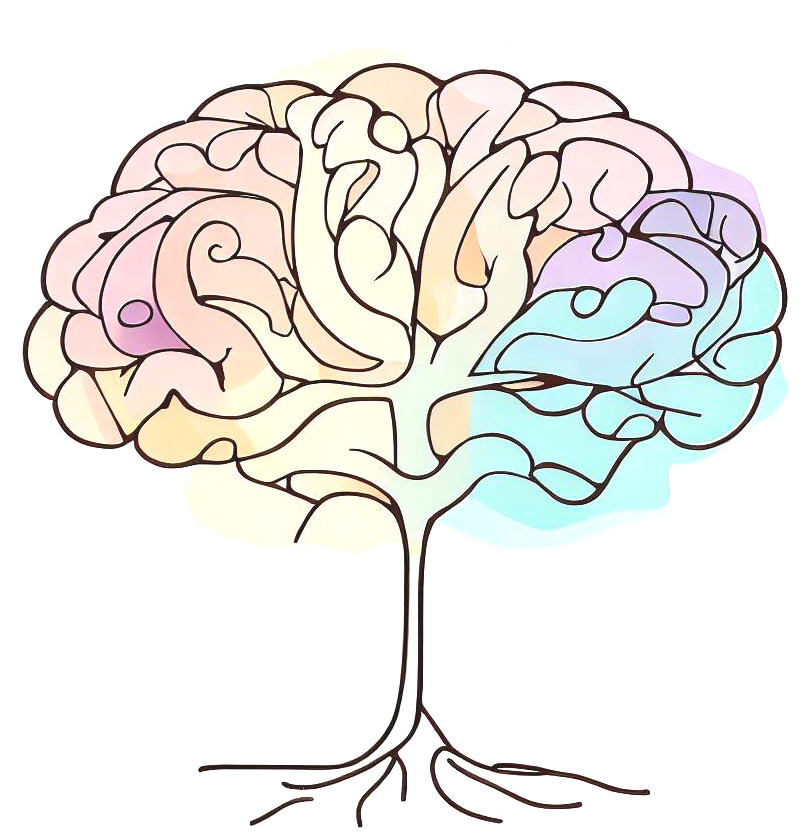
\includegraphics[height=7cm]{images/tree-cover} 

\vspace{4cm}
\tiny{
Первое издание\\
(с ошибками и без дополнений)
}
\end{center}


\thispagestyle{empty}
\newpage
\thispagestyle{empty}  % to not have a page# here

\selectlanguage{russian}
% \backgroundsetup{scale=1,opacity=1,angle=0,contents={\includegraphics[width=\paperwidth,height=\paperheight]{eclipse.jpg}}}

\clearpage
% uncomment the line below to hide page number 
% \thispagestyle{empty}
\hfill

%\backgroundsetup{scale = 1, angle = 0, opacity = 0.02, contents = {\includegraphics[width = \paperwidth, height = \paperheight] {images/mountains.pdf}}}
%\BgThispage


\addto\captionsrussian{ 
}
% so the table of contents itself is not shown in the table of contents
\begin{KeepFromToc}
  \tableofcontents
\end{KeepFromToc}

\backgroundsetup{scale = 1, angle = 0, opacity = 0.9, contents = {\includegraphics[width = \paperwidth, height = \paperheight] {images/camel}}}
\BgThispage


\thispagestyle{empty}  % hide page number
\newpage
\thispagestyle{empty}

\pagenumbering{arabic}  % so the second page begins with #1

%\chapter{asdsads}


\section*{Зебра, которая не заблудилась}
\yinipar{\color{red}O}днажды, давным давно, глубоко в африканской саванне, жила была зебра.




\newpage
\section*{Верблюд, который не заблудился}

\newpage
\section*{Медведь, который не заблудился}



% this is the back-cover of the book
\cleartoverso
%\cleartorecto 
% \cleartoevenpage
% \clearpage
\thispagestyle{empty}  % to not have a page# here


\section*{Другие книги нашего издательства}
% \vspace{2cm}

\begin{table}[h]
\begin{tabular}{ccc}

\includegraphics[height=4cm]{images/cava-bien} & 
\includegraphics[height=4cm]{images/suslik} & 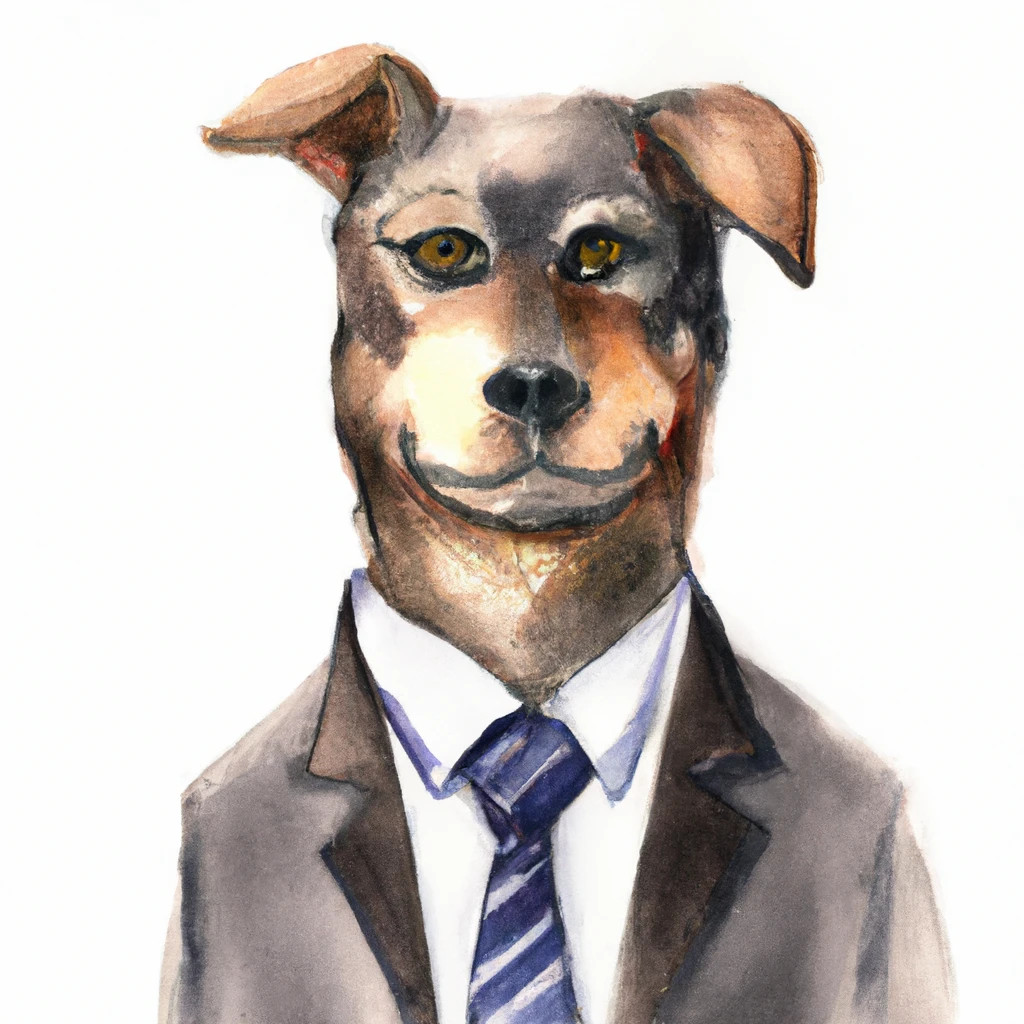
\includegraphics[height=4cm]{images/sobachevich}             \\
 Сова Бьен    &  Сусленский суслик        &   Господин Собакевич            \\
   &  & \\
            &          &              \\
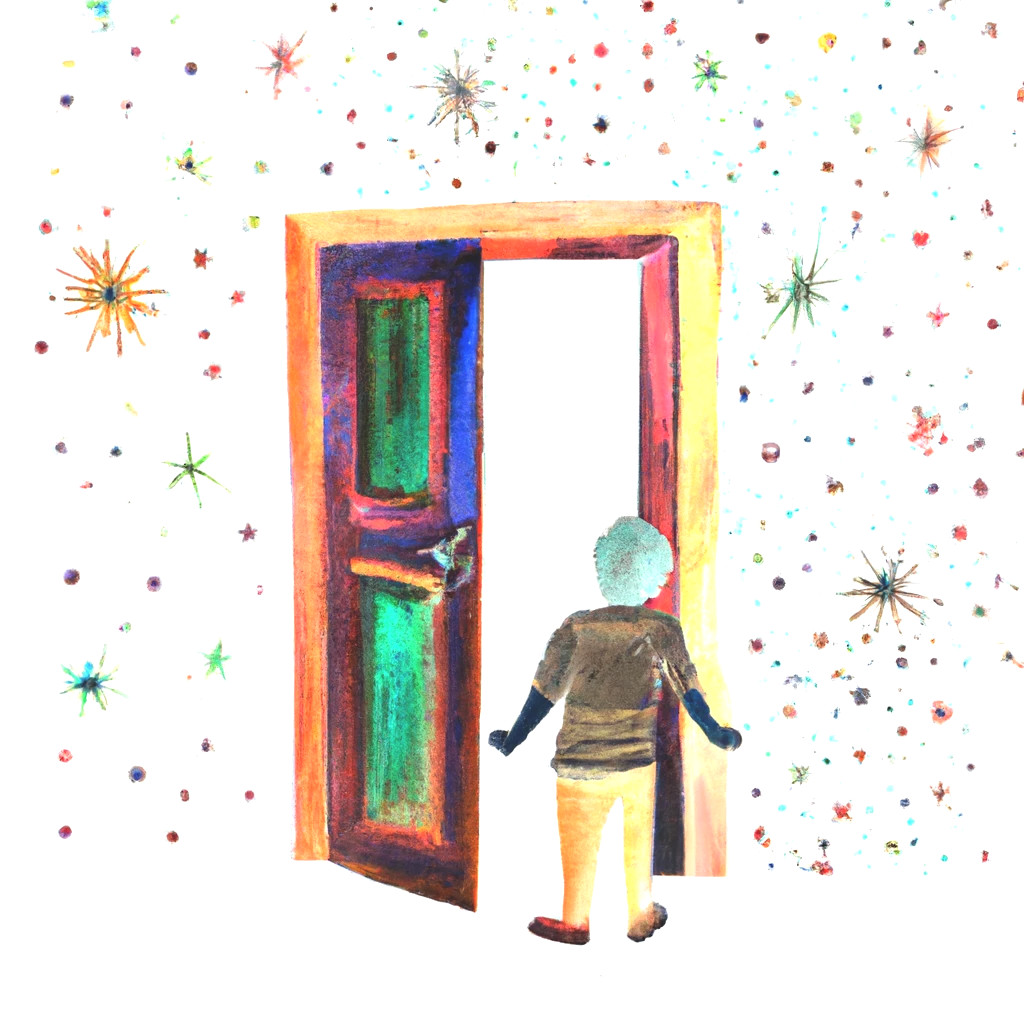
\includegraphics[height=4cm]{images/cosmoroom} & 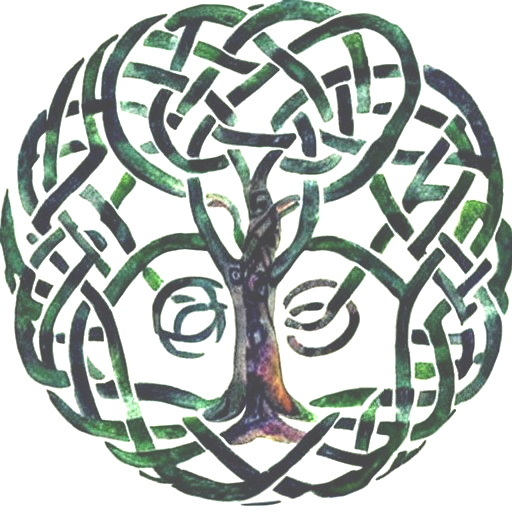
\includegraphics[height=4cm]{images/tree-cover-one} & \includegraphics[height=4cm]{images/razukrashki.jpg}             \\
 Окно в космос       &  Книга добрых детей    &     Разукрашки \\    
        &      &     Дваукрашки \\
        &      &     Триукрашки \\
\end{tabular}
\end{table}

\subsection{Автор и обратная связь}
\hspace{-1cm}
\noindent
\begin{tabular}{p{12cm}p{2cm}}
\footnotesize{Этот сборник стихов из частично-восстановленного архива, найденного среди развалин архаического вычислительного центра, на дне озера $0x\Sigma \alpha \phi^4_5\bigoplus$. Исходя из метаданных, стихи были написаны в первой половине XXI века Ручной эпохи Досингулярной эры. Предполагаемое имя автора Papa de la M{\"u}nchen, или Папа де ла Мюнхен, или Папа Мюнхенксий (возможно искажение транслитерации). % Среди блоков данных был найден и фрагмент который не поддавался текстовой интерпретации, мы прилагаем его в виде двухмерной монохромной матрицы. Остальные двухмерные матрицы в сборнике были сгенерированны нами, исходя из контекста.
О неточностях и ошибках сообщайте в Департамент Интерпретаций: alex\faIcon{cat}railean.net.} & \hspace{-5mm}\raisebox{-2.2cm}{ 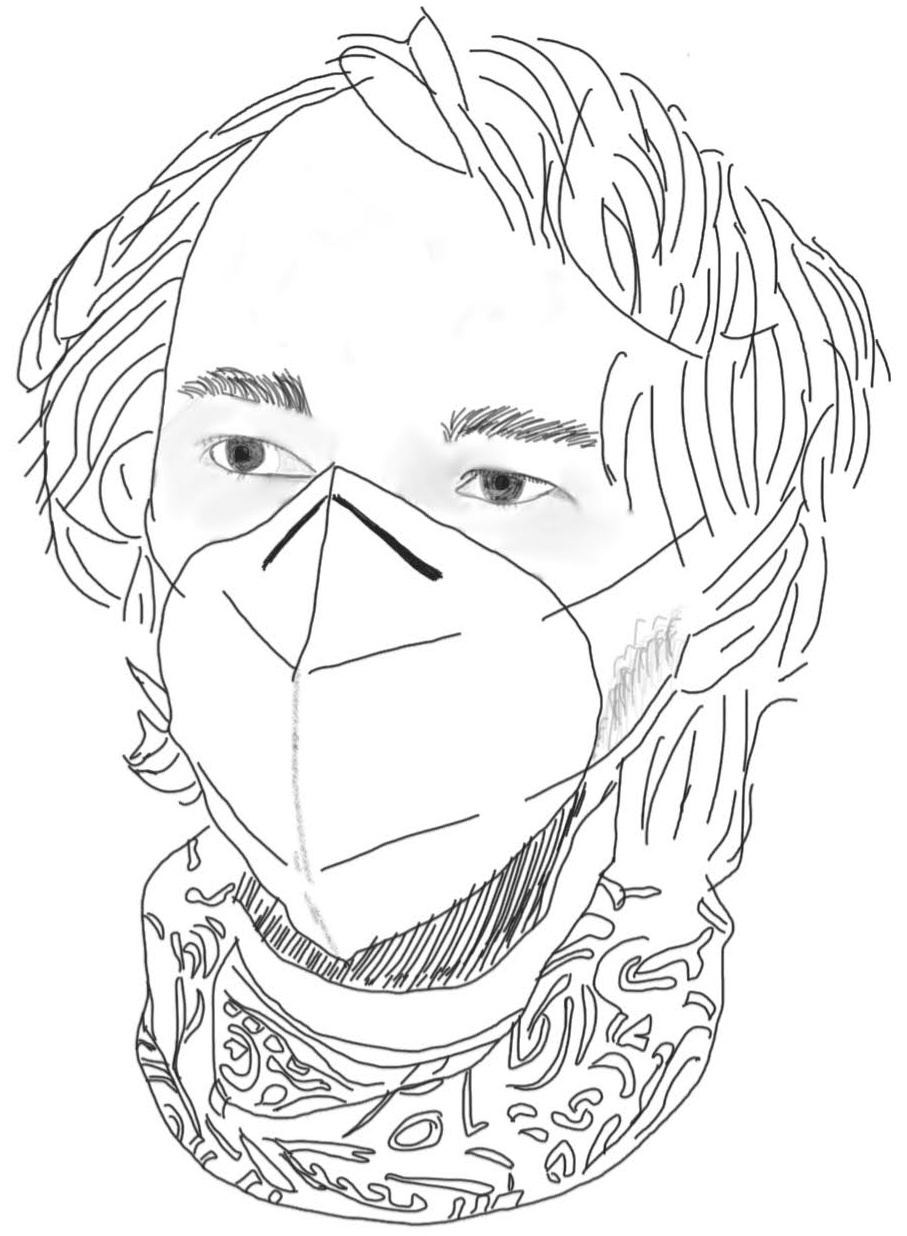
\includegraphics[height=2.5cm]{images/maskavatar-trimmed.jpg}} \\


\includegraphics[height=1.3cm]{images/payments/qr-btc.pdf} \hspace{0.5cm} 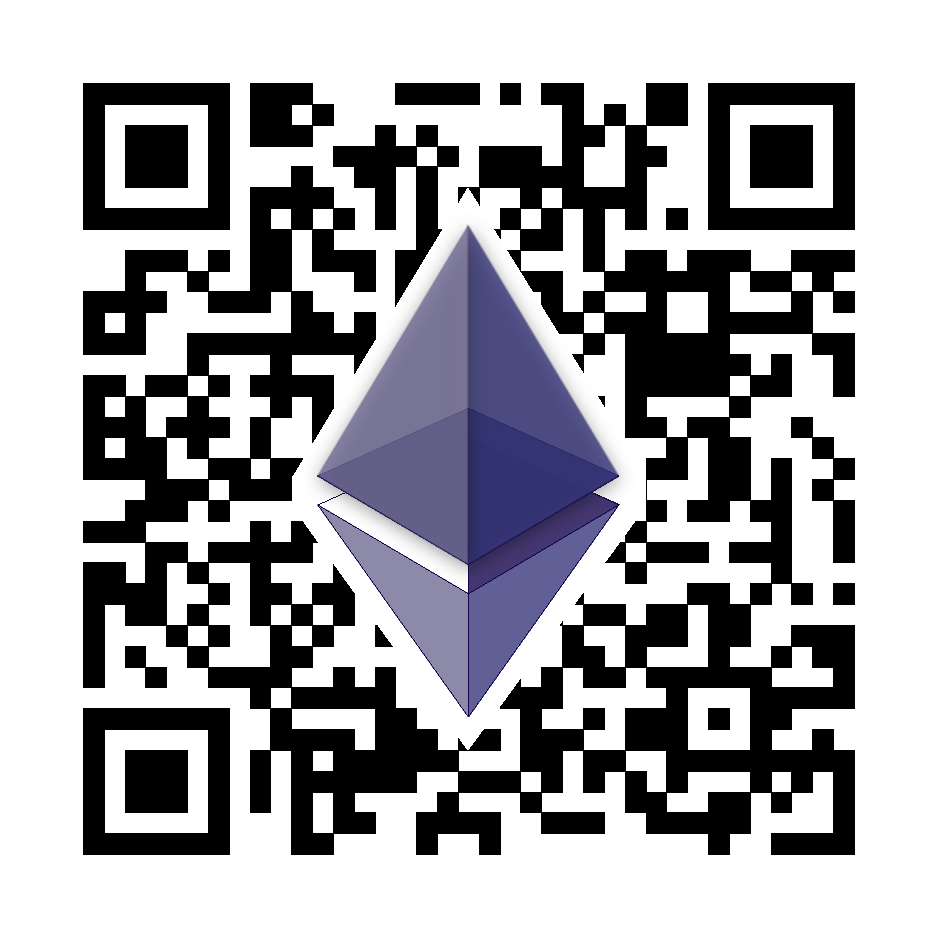
\includegraphics[height=1.3cm]{images/payments/qr-eth.pdf} \hspace{0.5cm} \href{https://paypal.me/ralienpp}{
\includegraphics[height=1.3cm]{images/payments/qr-paypal.pdf}} \hspace{5cm} \href{https://creativecommons.org/licenses/by-sa/4.0/}{\includegraphics[height=0.3cm]{images/cc-by-sa.eps}}&
\end{tabular}

\end{document}


